\documentclass{article}
\usepackage[utf8]{inputenc}
\usepackage{amsthm, amsmath, amssymb, mathrsfs}
\usepackage{tikz}
\usepackage{graphics}
\usepackage{float}

\newtheorem{recap}{Recapitulation}

\title{Master 2 CSMI : EDP2\\Rapport TP2\\Résolution numérique de Saint-Venant}
\author{Romain Vallet}

\begin{document}

\maketitle

\subsubsection*{1.}

Voici le graphique du solveur de Riemann :

\begin{figure}[H]
    \centering
    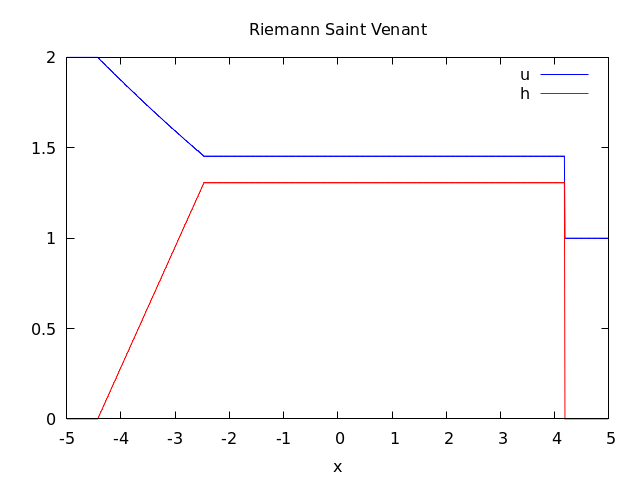
\includegraphics[scale=0.5]{figure/riemann.png}
    \caption{Solveur de Riemann}
\end{figure}

\subsubsection*{2.}

\subsubsection*{3.}

Nous pouvons poser comme conditions au bords :
\[ \left\{ \begin{matrix} 
    u_0^n = - u_1^n \\
    h_0^n = h_1^n \\
    u_N^n = - u_{N-1}^n \\
    h_N^n = h_{N-1}^n
\end{matrix} \right. \]

\subsubsection*{4.}

\subsubsection*{5.}

Nous posons $A(w) = f'(w) = \begin{pmatrix} 0 & 1 \\ -u^2+gh & 2u \end{pmatrix}$

Avec les valeurs propres de $A(w)$ : $\lambda_1(w) = u - \sqrt{gh}$ et $\lambda_2(w) = u + \sqrt{gh}$.

Nous posons la vitesse $\lambda = max(\rho(A(w_L), \rho(A(w_R)))) = max(|u_L|+\sqrt{gh_L}, \, |u_R|+\sqrt{gh_R})$

Le flux de Rusanov devient :
\begin{eqnarray*}
    f(w_L, w_R) &=& \frac{f(w_L) + f(w_R)}{2} - \frac{\lambda}{2} (w_R - w_L) \\
\end{eqnarray*}

\end{document}
